\documentclass[../main/thesis.tex]{subfiles}
\begin{document}
\newpage
%% my chapter 1 content
\chapter{Testing and Characterization of the 3DMiMic Detector}
\label{3dmimic}

\section{Radiation Detectors}
\label{t-detector}
A radiation detector records interactions between incoming radiation and the detector. These interactions could be electrical, chemical, light- or heat-based. Detectors can be based on many different materials, including gas chambers, semiconductors, crystals, and liquid.\comm{\citep[chap. 9]{Thorsteinsen}} In a simple radiation detector a single particle interacts with the detector, resulting in an electric charge appearing inside the detector. This charge is typically collected by setting up an electric field inside the detector, which causes positive and negative charge to flow in opposite directions, forming an electric signal. This signal could be measured as a current (current mode), voltage (mean square voltage mode), or a charge (pulse mode). \citep[chap. 4]{Knoll}

Pulse mode is the most common readout mode because the measurement records each individual quantum of radiation. Pulse mode is therefore required when attempting to measure the energy of individual radiation events. The charge generated in the detector is usually integrated over a certain period of time. Pulse mode however does not work well at very high event rates as the time between events becomes too short to analyse the data. Current mode measures the average current over many events, therefore loosing the amplitude and timing information of individual events, but allowing for measurement with high event rates. Mean square voltage mode works much like current mode, but the output signal will be more dependent on the charge per event, making this mode more useful for mixed radiation environments. \citep[chap. 4]{Knoll}

%pulse height spectra, energy resolution, efficiency, dead time


%Dosimeter, microdosimeter?

\subsection{Semiconductor Detectors}
\label{t-semi}
Semiconductor diode detectors, also called simply semiconductor detectors or solid-state detectors, are radiation detectors employing semiconductor diodes as the basic detection medium. Silicon is the most common material used, but germanium detectors are superior for gamma-ray measurements. Semiconductor detectors offer energy resolutions that are superior to other radiation detectors in addition to small size and fast timing characteristics. A big drawback is that they are degraded by radiation-induced damage during normal use. \citep[chap. 11]{Knoll}

Charged particles passing through a semiconductor detector create electron-hole pairs along the particles path. By setting up an electric potential across the diode, there will be an electric field present that will cause the holes to drift in the same direction as the electric field vector, and the electrons in the opposite direction. By monitoring one of the diodes sides, a pulse is measured as the charge from either the holes or the electrons (depending on which side is measured) is collected. 

A semiconductor detector, like other diodes, can be forward biased (positive potential on p-side) or reverse biased (positive potential on n-side). It is possible to operate a semiconductor detector without external bias, but it will perform poorly as the electric field across the junction will be too weak to read out the charge carriers before many are lost. Applying forward bias to the detector reduces the electric field even further, while reverse bias increases it. Another important factor is that reverse bias increases the depletion region, which is also the active volume of the detector. \comm{This is the main reason for reverse bias being the dominant choice for radiation detectors.}\citep[chap. 11]{Knoll}

%Tran phd fig 1.3?

%%XXX p-i-n

%%%XXX More details and figures

\section{Semiconductor Characterization}
\label{t-char}

\subsection{Capacitance-Voltage Measurements}
\label{t-cv}
\gls{CV} profiling is a semiconductor characterisation technique that is much used to find doping- and defect densities in semiconductor junctions. The technique relies on the fact that the width of a reverse biased depletion region depends on the applied voltage. The small signal capacitance is dependent on both the doping density and width of the depletion region. \gls{CV} profiles are made by measuring the capacitance while sweeping over a voltage range. The doping density is found from the slope of a C-V curve or a $1/C^2$-V curve. \citep[chap. 2]{Schroder}

There are multiple ways to measure capacitance. A simple method is to supply a known current, and measure how fast the voltage across the capacitor rises. This method assumes an ideal capacitor, and is therefore inaccurate for a real capacitor. A more accurate method is to supply an AC signal to the \gls{DUT} and measure the AC current and voltage. A high frequency signal ($\sim$10 MHz) will be better for measuring dynamic performance, while a low frequency signal ($\sim$10 kHz) is better to find quasistatic characteristics. The capacitance is calculated from the frequency, current, and voltage. 
%%XXX equation?

%https://en.wikipedia.org/wiki/Capacitance_meter
%http://www.planetanalog.com/document.asp?doc_id=527457
%Paper we got in lab

\subsection{Current-Voltage Measurements}
\label{t-iv}
\gls{IV} characterization is observation of the current through a device when sweeping over the voltage across it. This can be used to find basic electrical parameters for the device. This includes leakage current, resistance, cut-in voltage, breakdown voltage, saturation voltage, and hysteresis. 

\section{3DMiMic}
\label{3d-3d}

\begin{figure}%[h]
	\centering
	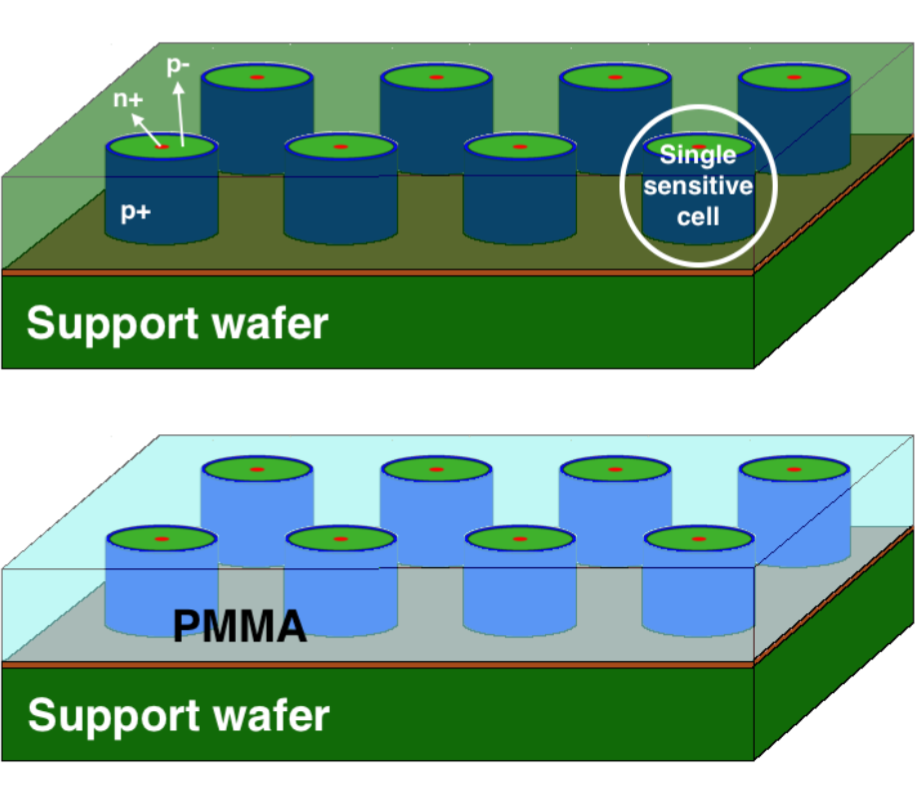
\includegraphics[width=0.6\textwidth]{3dmimic.png}
	\caption{Presentation sketches of the 3DMiMic detector, shown without and with PMMA. \citep{Trento2015}}
	\label{fig-3dmimic}
\end{figure}

Si-3DMiMic, or simply 3DMiMic, is a silicon-based 3D mini and micro-dosimeter being developed by SINTEF MiNaLab in Oslo, but was invented and ordered by Professor Anatoly Rozenfeld from the Centre for Medical Radiation Physics at the University of Wollongong. The detector is made to mimic the response of biological tissues to ionizing radiation on a cellular and sub-cellular level, and consists of an array of more than a thousand cylindrical p-i-n diodes (see figure \ref{fig-3dmimic}). Each diode, or cell, is made of a thin n+ core cylinder, a circular p+ trench some micrometers out, and in some cases a n+ guard ring further away from the core (see figure \ref{fig-3dmimic-top-side}). There are multiple versions of the detectors, with differences including presence of n+ guard ring, size of cell, and structure. The silicon between the different cells should be etched away and replaced with tissue equivalent \gls{PMMA}, but this has not been attempted by SINTEF yet as of the time this thesis is written. This should be done because \gls{PMMA} produces secondary radiation in a very similar way to how tissue does, unlike silicon, due to the mass numbers of the atoms. 
%some are 50x50

%Each diode, or cell, is made of a 3 $\mu$m diameter n+ core cylinder, a 2 $\mu$m thick p+ trench about 10 $\mu$m further out, and a 4 $\mu$m thick n+ ring about 20 $\mu$m outside the core. The silicon between the different cells has been etched away and replaced with tissue equivalent \gls{PMMA}. %Need to double check all this later, I have contradicting sources

Figure \ref{fig-3dmimic-side} show a "3D" layout with the n+ core cylinder and the p+ trench going all the way through the bulk, and a planar n+ guard ring. There also exist designs with either or both the n+ core and p+ trench made planar. Figure \ref{fig-3dmimic-top15} shows the smallest, "15 $\mu$m", layout of 3DMiMic from above with a size scale. The larger, "30 $\mu$m", layout has a roughly 25 \% larger radius than the "15 $\mu$m" layout. The detectors with the smaller diodes have 50x50 cells, while the larger variant has 32x33 cells. Images of some of the different layouts can be found in Appendix \ref{a-3dmimic-layout}.

%%XXX doublecheck 32x33 again

%\begin{figure}%[h]
%	\centering
%	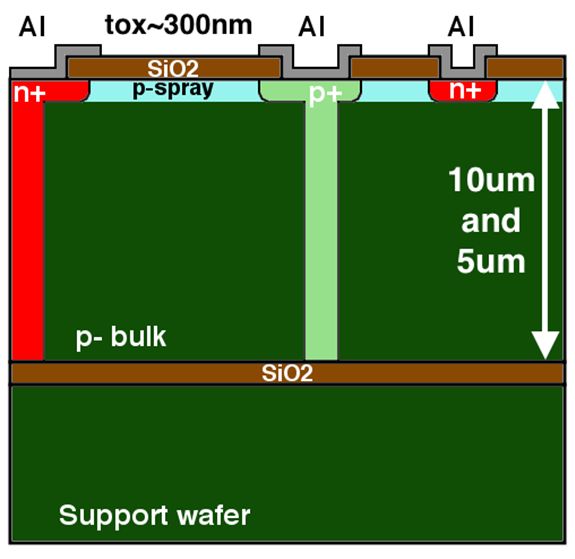
\includegraphics[width=0.5\textwidth]{3d-side.png}
%	\caption{Layout of 3DMiMic design with 3D n+ core and 3D p+ trench. \citep{Marco}}
%	\label{fig-3dmimic-side} %need to check permission
%\end{figure}

\begin{figure}
	\centering
	\begin{subfigure}{.5\textwidth}
		\centering
		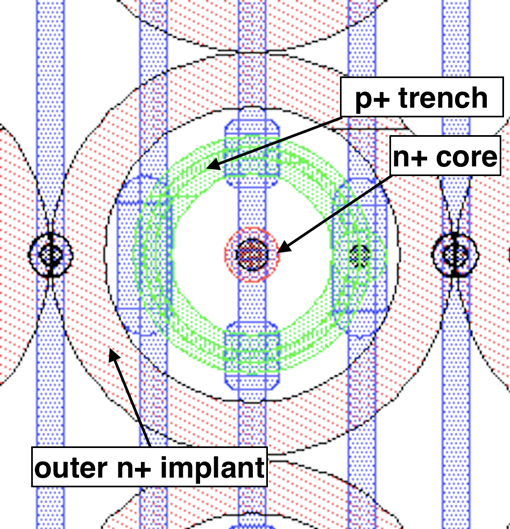
\includegraphics[width=.9\linewidth]{3d-top.png}
		\caption{Top view with guard ring present.}
		\label{fig-3dmimic-top}
	\end{subfigure}%
	\begin{subfigure}{.5\textwidth}
		\centering
		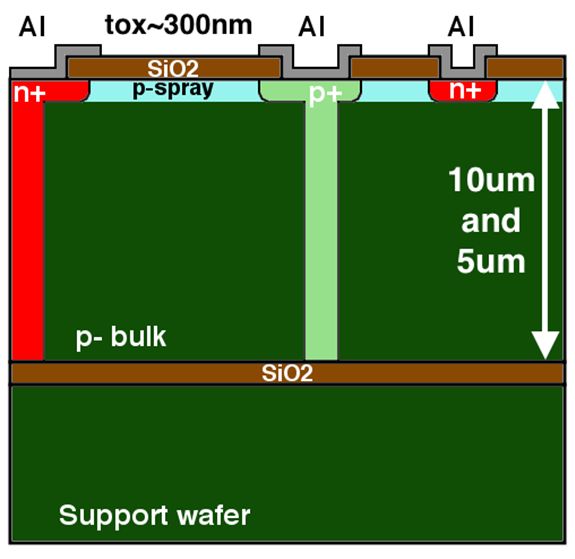
\includegraphics[width=\textwidth]{3d-side.png}
		\caption{Side view with 3D n+ core, 3D p+ trench, and planar n+ guard.}
		\label{fig-3dmimic-side} %need to check permission
	\end{subfigure}
	\caption{Layout of a 3DMiMic cell. \citep{Marco}}
	\label{fig-3dmimic-top-side}
\end{figure}


\begin{figure}[h]
	\centering
	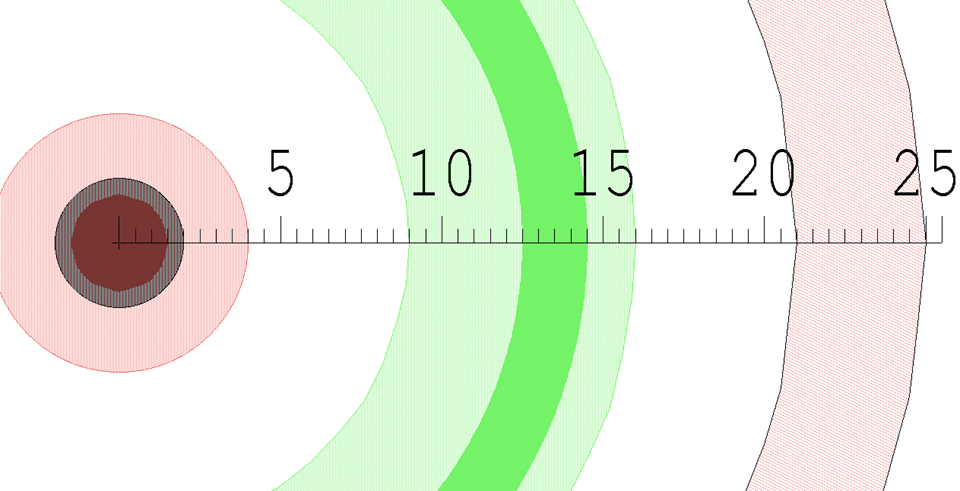
\includegraphics[width=0.7\textwidth]{3d-top15.png}
	\caption{Smallest, "15 $\mu$m", layout of 3DMiMic seen from above. Distance scale is in $\mu$m. \citep{Marco}}
	\label{fig-3dmimic-top15} %need to check permission
\end{figure}

In the main layout of 3DMiMic, all the n+ cores in a line is connected together. Every second line is also connected, leaving two channels (odd/even) for readout. When present, all the outer n+ rings are connected and can be read out if desired. A full die is shown in figure \ref{fig-3dmimic-die}, where the "+" pads are the n+ cores, the "G" pads are for the p+ trenches, the "GUARD" pads are for the cell guard rings, and the large square around the detector is a guard ring. There also exist other layouts, for example with all diodes connected together, readout in eight channels, and a larger design made to be bump bonded to a Medipix chip (see section \ref{e-medipix}). 

\begin{figure}%[h]
	\centering
	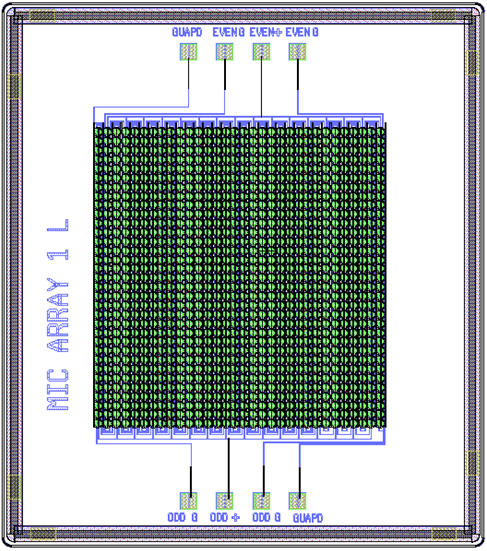
\includegraphics[width=0.6\textwidth]{3d-die.png}
	\caption{Layout of a full 3DMiMic die, showing bonding pads and the guard ring outside the active area. \citep{Marco}}
	\label{fig-3dmimic-die} %need to check permission
\end{figure}

Even though the odd/even readout scheme contains two channels, it does not provide any spacial information, as both channels cover the whole active area of the detector. The reason for this layout is to notice if a particle track goes through multiple adjacent cells. If both readout channels are triggered at the same time, this was not a single event, as it will look if all cells are read in a single channel.

\subsection{3DMiMic Response to Radiation}
Table XXXX from \citep{Samnoy} show the expected signal strength in number of electrons from a \gls{MIP} to a Carbon ion in the Bragg peak. 

\section{I-V Measurements of 3DMiMic Detectors on Wafer}
\label{3d-IV}
\gls{IV} measurements of seven 3DMiMic wafers where performed in the cleanroom at SINTEF MiNaLab in Oslo by Øyvind Lye and Andreas Tefre Samnøy in May 2016. These seven wafers have been produced with different designs and fabrication processes. Each wafer has 104 detectors with odd/even readout, 6 detectors with single channel readout, and several other experimental layouts. The detectors had to be tested with manual needle placement, as the designs are too different to use an automatic system with a probe card. The wafer is held in place on a stand using vacuum, and the stand can be moved in the horizontal plane. The needles can be manually placed at the desired location, and the position can be fine-tuned in Cartesian space using screws. The cell n+ guard ring was not connected on the detectors where it is present. This was done because it would require a separate test setup for the detectors with the ring, which would increase the time needed for the measurement. A total of 580 detectors were measured. 

\section{Detector Interface PCB}
\label{3d-pcb}
A \gls{PCB} was designed to interface 3DMiMic to the supply and readout electronics. This is described in detail in appendix \ref{a-pcb}.

\section{Wire Bonding}
Wire bonding the detectors to the PCB was supposed to be performed by SINTEF, but they had problems with the wire bonder in June 2016 which would have led to another delay. To avoid this delay, three detectors glued to PCBs were picket up at SINTEF and brought to the cleanroom at Vestfold Innovation Park for wire bonding. The wire bonder was already loaded with 17.5 $\mu$m gold wire, and this was used even though it is thinner than necessary for the 3DMiMic detectors. Each connection was done with two parallel wires to have some redundancy in case of mechanical damage to the thin wires. The three detectors are numbered: S10-15 $\#$128 (MIC$\_$ARRAY$\_$3$\_$PSTOP$\_$L layout), S10-17 $\#$51 (MIC$\_$ARRAY$\_$1 layout), and S10-17 $\#$128 (MIC$\_$ARRAY$\_$3$\_$PSTOP$\_$L layout). See appendix \ref{a-3dmimic-layout} for the differences in the wafers and layouts.
See appendix \ref{a-pcb} for bonding schematics. 

\section{I-V Measurements of 3DMiMic Detectors on PCB}

\section{C-V Measurements of 3DMiMic Detectors}

\section{Radiation Measurements with Americium source}


\end{document}